\documentclass[letterpaper, 11pt]{article}
    \usepackage[margin=0.9in]{geometry}
    \usepackage{graphicx, hyperref, enumitem, booktabs}
    \usepackage{cancel, verbatim}
    % rubber: set program xelatex
    \usepackage[calc,linalg,physics,stix]{bccho}

    \usepackage{tocloft}
    \usepackage{etoc}
    \usepackage[margin=1cm]{caption}
    \usepackage[labelformat=simple]{subcaption}
    \usepackage{float}
    % rubber: setlist arguments --shell-escape
    \usepackage{minted}
    \usepackage[linewidth=0pt]{mdframed}

    \definecolor{bg}{rgb}{0.95, 0.95, 0.95}
    \BeforeBeginEnvironment{minted}{\begin{mdframed}[backgroundcolor=bg]}
    \AfterEndEnvironment{minted}{\end{mdframed}}

    % \renewcommand{\thefigure}{\thesection.\arabic{figure}}
    \captionsetup[figure]{labelfont={it,bf}}
    \captionsetup[table]{labelfont={it,bf}}
    \captionsetup[subfigure]{labelfont={it}}
    \renewcommand\thesubfigure{(\alph{subfigure})}
    \captionsetup[subfigure]{format=hang}

    \newcommand*{\figref}[1]{\textbf{\figurename~\ref{#1}}}
    \newcommand*{\tblref}[1]{\textbf{\tablename~\ref{#1}}}

    \newcommand{\iic}{I$^2$C\xspace}
    \renewcommand{\v}[1]{\vec{#1}}

% Begin document

\begin{document}
    \begin{center}
        \large
        \textsc{\textbf{ELE 302 -- Independent Project Write-Up}} \vspace{5pt}

        \normalsize
        TJ Smith \hspace{1cm} Byung-Cheol Cho \\
        (Bench 207) \vspace{5pt}

        \emph{Due May 19, 2017}
        \normalsize
    \end{center}

\section{Overview}
The aim of this project was to build a robot capable of playing basic ping pong. Prior to beginning this project, we established four ideal objectives for the end product:
\begin{enumerate}[label=\textbf{\arabic*.}]
    \item Track a ping pong ball, estimate its trajectory and predict the location where the ball will land
    \item Determine (1) when it is the robot's turn to hit the ball and (2) when the ball will hit the net or leave the playing area
    \item Move the robot to the required location before the ball bounces twice and hit the ball back over the net
    \item Avoid leaving the playing field (area enclosed by table and net)
\end{itemize}
By Demo Day, we had implemented the hardware and software to achieve objectives 1, 3 and the first half of objective 2, and we had the capability of achieving the remainder of the objectives had we decided to implement them in software.

We used two Pixy cameras (CMUcam5) placed a fixed distance apart on the robot to triangulate the location of a bright red ball in three-dimensional coordinates. Once the camera system had collected enough data points to accurately predict all future positions of the ball until the second bounce, the robot moved to a location where the ball would bounce to the center of a paddle attached to its side, and provided a brief flick to the paddle to return the ball.

The speed and flexibility of movement we needed (we had to move up to 3 feet in less than half a second) required us to abandon the chassis used for our previous speed control and navigation assignments and adopt the large and powerful omni-wheel drive used by Ethan Gordon and Luke Pfleger in 2016. We used an accelerometer and gyroscope for dead reckoning of position (we could no longer use wheel rotation tracking because of slippage). In addition, we continued to use the PSoC 5LP because of its extensive motor control capacity (we required four PWM modules) while adding a Raspbery Pi 3 because of the intensive computation we expected to require for ball tracking and trajectory estimation.

\section{Theory}
\subsection{Stereo vision}
We used a pinhole camera model for our Pixy cameras. Under this model, points in 3-D world coordinates are projected onto an imaging plane using homogenous coordinates. In the simplified case when the camera is at the origin pointing in the positive $z$ direction (i.e. the image plane is at $z=1$), we convert from world coordinates $(x, y, z)^T$ to image coorinates $(m, n)^T$ using basic linear algebra. First, we define $\paren{x', y', z'}^T$ as follows:
\begin{align*}
    \pmat{x' \\ y' \\ z'} &= \pmat{f_x & 0 & c_x \\ 0 & f_y & c_t \\ 0 & 0 & 1} \pmat{x \\ y \\ z} \\
    \intertext{The $3\times 3$ matrix is known as the \textbf{camera intrinsic matrix}, $F$, with entries $f_x$ and $f_y$ that represent the scale of conversion between world units and pixel units, and $c_x$ and $c_y$ that are the horizontal and vertical offsets of the image origin in pixels. Since these are all parameters internal to the camera, they are known as intrinsic parameters. Typically, $c_x$ and $c_y$ correspond to half of the width and height of the output image respectively. Then, to convert to image coordinates we simply divide by the $z'$-component:}
    \pmat{m \\ n} &= \pmat{ x' / z' \\ y' / z' }
\end{align*}
Concisely, we can write $\vec{w}_h \equiv F \vec{w}$ where $\vec{w}_h = (m, n)^T$ and $\vec{w} = (x, y, z)^T$, and $\equiv$ represents the process of dividing by the third component. If the camera is located at a point $\vec{p}$ from the origin, we can simply modify this equation to read $\vec{w}_h \equiv F(\vec{w}-\vec{p})$.

The problem with position estimation with one camera is that this perspective projection is not reversible (the input has three degrees of freedom, while the output only has two), so we need some additional source of positional information in order to recover the third degree of freedom. We briefly considered using a single camera (for simplicity) and the observed size of the ball, since linear dimensions should scale with $1/z$ with distance from the camera, while the area should decrease with $1/z^2$. However, we quickly switched to using two cameras because (1) at reasonable distances (even as close as three feet away from the camera), the observed size of the ball was too small (on the order of tens of pixels) that it would have produced unacceptable granularity in our depth measurements; and (2) the image processing of the Pixy camera was noisy and caused the area to fluctuate too much, producing noise in depth that would have been unacceptable for trajectory estimation.

Given image coordinates from two identical cameras with a known translational separation (and to simplify our calculations, no rotation), we can recover the original $z$-component in world coordinates by solving
\begin{align*}
    &\lb{
        \v{w}_{h1} &\equiv F\paren{\v{w}-\v{p}_1} \\
        \v{w}_{h2} &\equiv F\paren{\v{w}-\v{p}_2} \\
    } \\
    \implies &\pmat{m_1 - m_2 \\ n_1 - n_2 \\ z} \equiv F\paren{\v{p}_2 - \v{p_1}} \\
    \intertext{If there is only an $x$-displacement between the two cameras, we can estimate $z$ directly from only the horizontal disparity in the images:}
    \implies &z = \frac{f_x t_x}{m_1 - m_2}
\end{align*}
where $t_x = \paren{\v{p}_{2} - \v{p}_{1}}_x$.

The convention for camera coordinates typically has $z$ along the principal axis of the camera, but since our camera was mounted on the front of the robot, we performed a basic coordinate transform so that $z$ was vertical (normal to the ground):
\begin{align*}
    x\sub{world} &= x\sub{camera} & y\sub{world} &= z\sub{camera} & z\sub{world} &= y\sub{camera}
\end{align*}
For trajectory estimation and prediction, we used only world coordinates to avoid confusion.

It is important to note that the Pixy camera is not an ideal pinhole camera. Critically, it exhibits radial distortion. We attempted correcting for this by calibrating using MATLAB's camera calibration methods (e.g. the \verb|cameraCalibrator| app), but we found little significant improvement in position estimation, and the small position differences from the distorted image and coordinates were sufficient for our purposes.

\subsection{Trajectory estimation and prediction}
Trajectory estimation is the process of performing statistical estimation of kinematic parameters, such as initial position and velocity in all three spatial dimensions, and acceleration in the world $z$-axis. Among our many design iterations, we also estimated the coefficient of restitution from our observed data. We approached trajectory estimation with a linear regression model with various modifications, and then used the estimated kinematic parameters to estimate the time and location of bounces (i.e. perform trajectory prediction). We decided to use regression instead of finite difference methods because we expected our stereo ball tracking data to be rather noisy (finite differences tend to amplify high-frequency noise).

We divided our model of the ball's trajectory into the global $x$, $y$ and $z$ coordinates (relative to the robot, since we simplified our problem by tracking the ball only while the robot was stationary). For the $x$ and $y$ coordinates, we performed simple linear regression over all detected ball positions:
\begin{align*}
    x &\sim \beta_{x0} + \beta_{x1}t & y &\sim \beta_{y0} + \beta_{y1}t
\end{align*}
For the $z$ coordinate, we performed linear regression with quadratic time features:
\begin{align*}
    z &\sim \beta_{z0} + \beta_{z1}t + \beta_{z2}t^2
\end{align*}
$\beta_{x0}$, $\beta_{y0}$ and $\beta_{z0}$ all represent the initial positions (at $t=0$); $\beta_{x1}$, $\beta_{y1}$ and $\beta_{z1}$ all represent the initial velicities (at $t=0$); and $\beta_{z2}$ represents the acceleration due to gravity.

All of these regression models can be written as $\v{Y} \sim \mat{X} \v{\beta}$ where $\mat{X}$ is the $n\times d$ feature matrix: for the $x$ and $y$ coordinates, $\mat{X}$ consists of a column of ones, and a column for $t$; for the $z$ coordinate, $\mat{X}$ consists of a column of ones, a column for $t$, and a column for $t^2$. Then, assuming that $n\ge d$ so that $\mat{X}$ is not rank-deficient, by ordinary least squares (OLS) we have a simple formula for the regression coefficients, $\v{\beta}$:
\[ \hvec{\beta}\sup{OLS} = \paren{ \mat{X}^T\mat{X} }\inv \mat{X}^T \v{Y}. \]

The $z$-coordinate regression model is, however, rather limited: since it represents a pure parabola, it cannot take bouncing into account. To overcome this, we implemented a transform mapping points from after a bounce back onto the original parabola to continue to improve our regression coefficients; this transform was based on the observation that the parabola after a bounce is a scaled version of the original parabola (see \figref{fig:bounce} below).

Specifically, the bounce height and duration are completely determined by the velocity of the ball after the bounce, so if $R$ is the coefficient of restitution (i.e. the ratio between energy after and before a bounce, or equivalently, between the maximum height before and after a bounce), the velocity after the bounce is scaled by $\sqrt{R}$, the height is scaled by $R$, and the duration of the bounce is scaled by $\sqrt{R}$ (since bounce duration is given by $2v\sub{init} - gt\sub{duration}$). Therefore, in order to rescale the data back to the first parabola, we reflect time points $t \mapsto t\sub{bounce} - \paren{t - t\sub{bounce}} / \sqrt{R}$ and scale $z \mapsto z / R$. This is demonstrated in \figref{fig:transform} below.

\begin{figure}[ht]
    \centering
    \begin{subfigure}[t]{0.48\textwidth}
        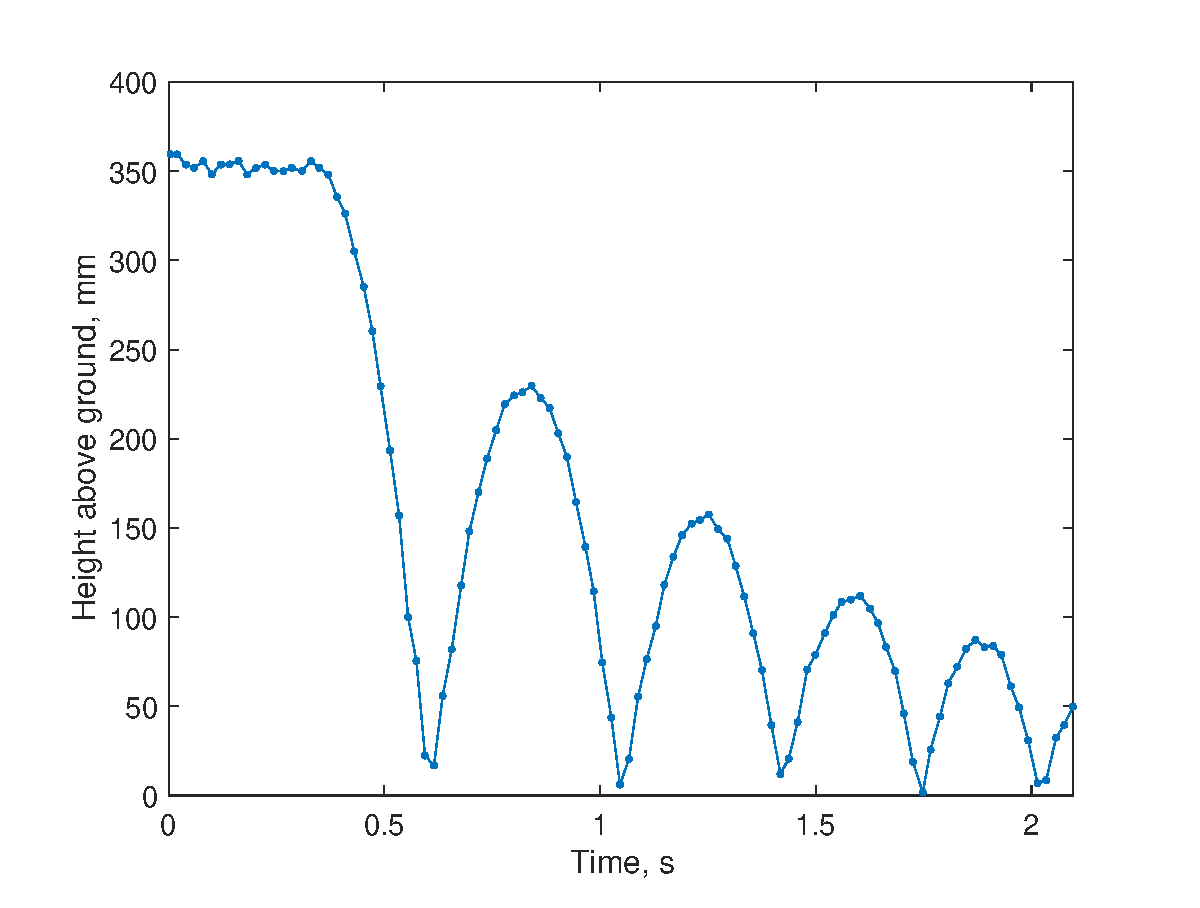
\includegraphics[width=\textwidth]{images/fig_bounce.eps}
        \caption{Plot of ball height over several bounces. The ball is dropped around $t = \SI{0.35}{\second}$.}
        \label{fig:bounce}
    \end{subfigure}\hfill
    \begin{subfigure}[t]{0.48\textwidth}
        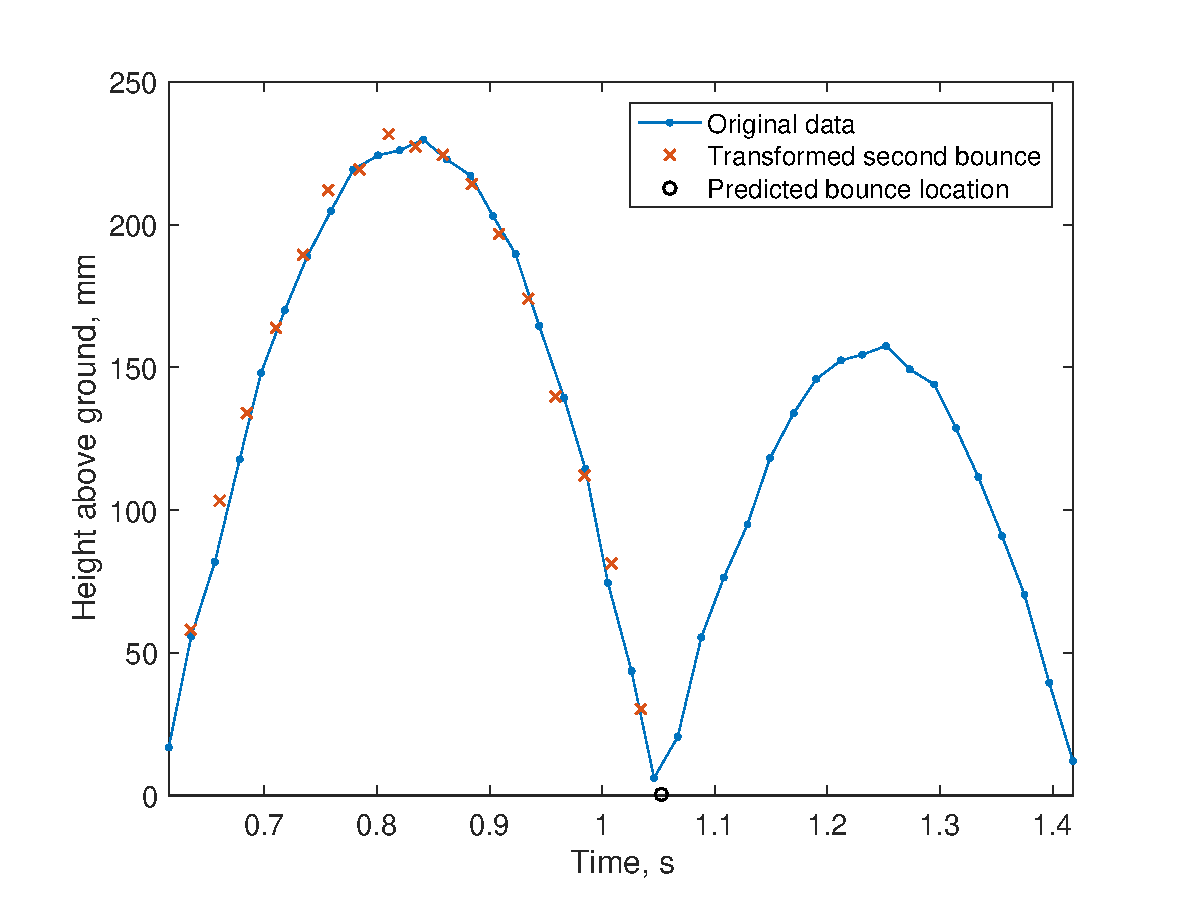
\includegraphics[width=\textwidth]{images/fig_transform.eps}
        \caption{Demonstration of the reflection and rescaling transform, using $R = 0.68$.}
        \label{fig:transform}
    \end{subfigure}
    \caption{\textbf{Kinematics of ball-bouncing.}}
\end{figure}

However, this introduced a new free parameter, $R$, that happens to be critical for accurate transformation. We could not estimate $R$ using linear regression, because the model was no longer linear: $z \sim \paren{\beta_0 + \beta_1 t + \beta_2 t^2} / R$. Thus, we were forced to either hard-code a value for the coefficient of restitution, attempt to minimize the mean-squared error among a range of $R$ values (since reasonable values of $R$ were between $0.2$ and $0.8$), or iteratively regress for better values of $R$ and $\v{\beta}$ using some form of block coordinate minimization. We initially attempted to implement the latter two algorithms, but in the late hours of Wednesday night / Thursday morning, something was wrong in our implementations, so we decided to hard-code a value of $R$ based on the surface and type of ball we were working with.

Finally, once the kinematic parameters were estimated, it was trivial to predict the location of the ball in global coordinates for any point in time in the future. Specifically, the landing location could be estimated by computing the roots of the $z$ polynomial, and by simple extension, the location of the ball at any height (since our paddle was vertically fixed) could be estimated using some more quadratic formulas.

\subsection{Omni-drive}
%TODO: TJ: give BC equations and BC typesets them

\clearpage
\section{Hardware}
\figref{fig:pics} shows photographs of the final product from various angles, annotated with important components
\begin{figure}[H]
    \centering
    \begin{subfigure}[t]{0.8\textwidth}
        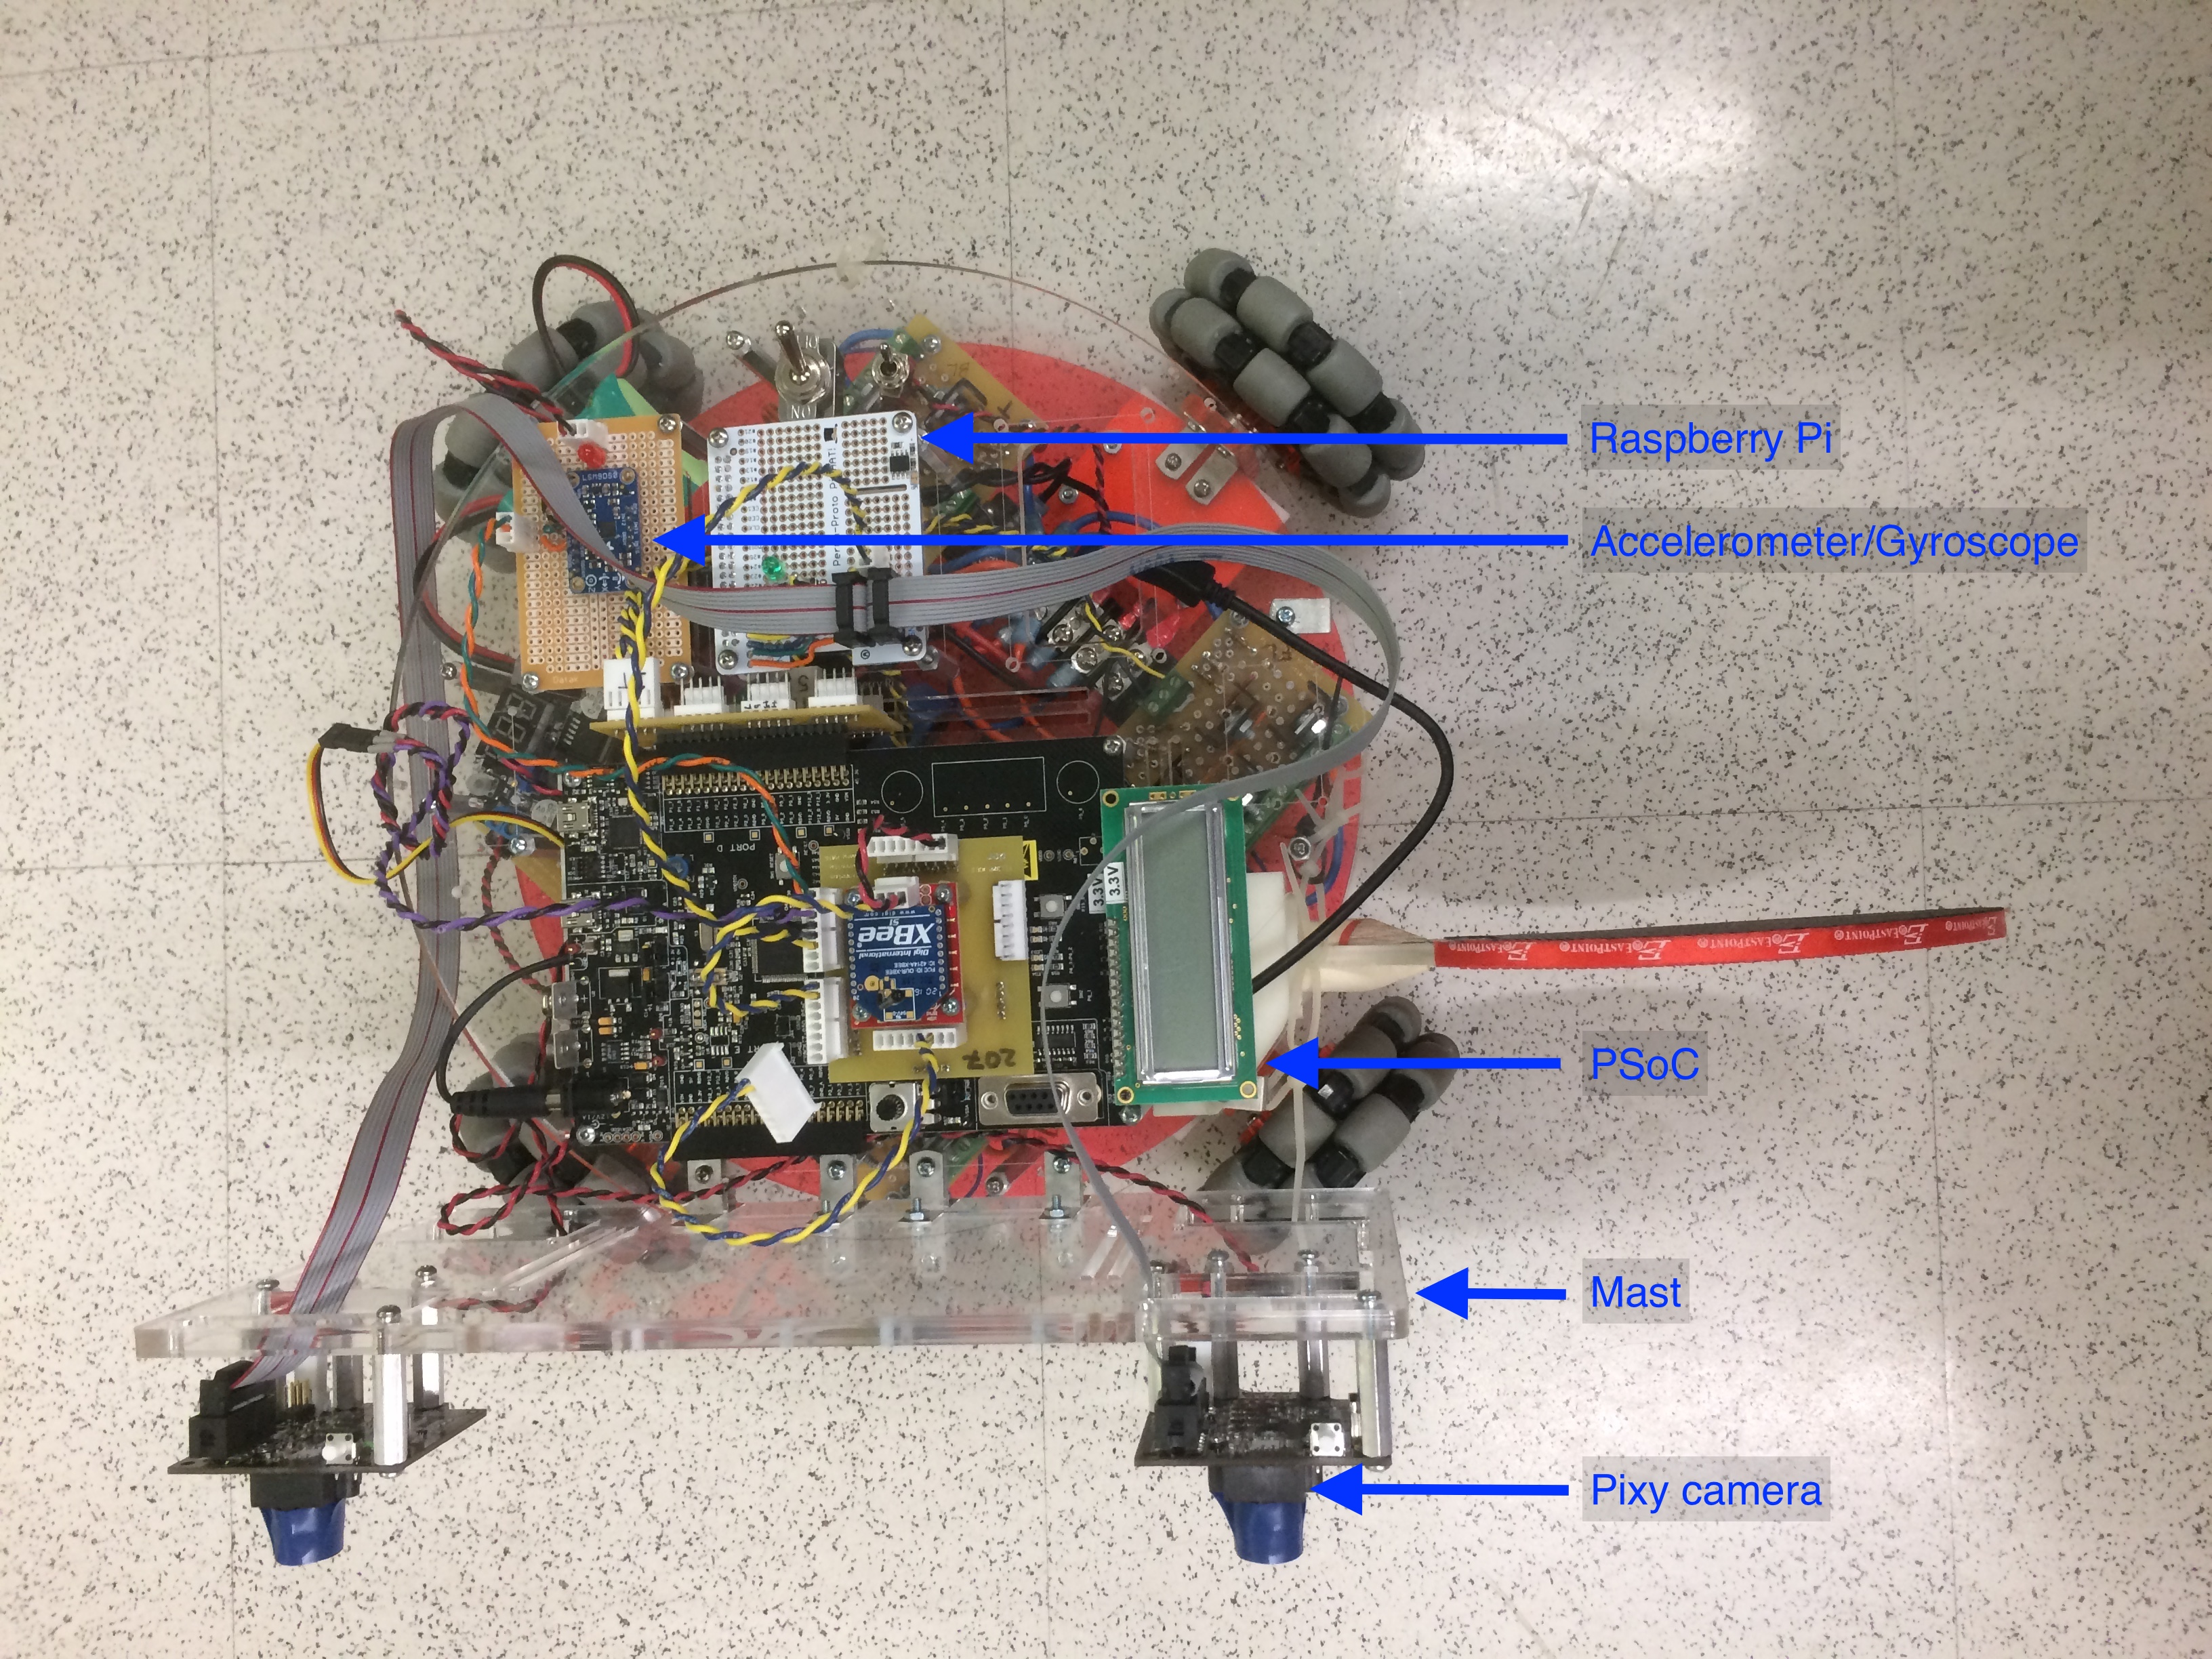
\includegraphics[width=\textwidth]{images/top.JPG}
        \caption{Top view.}
    \end{subfigure}

    \begin{subfigure}[t]{0.8\textwidth}
        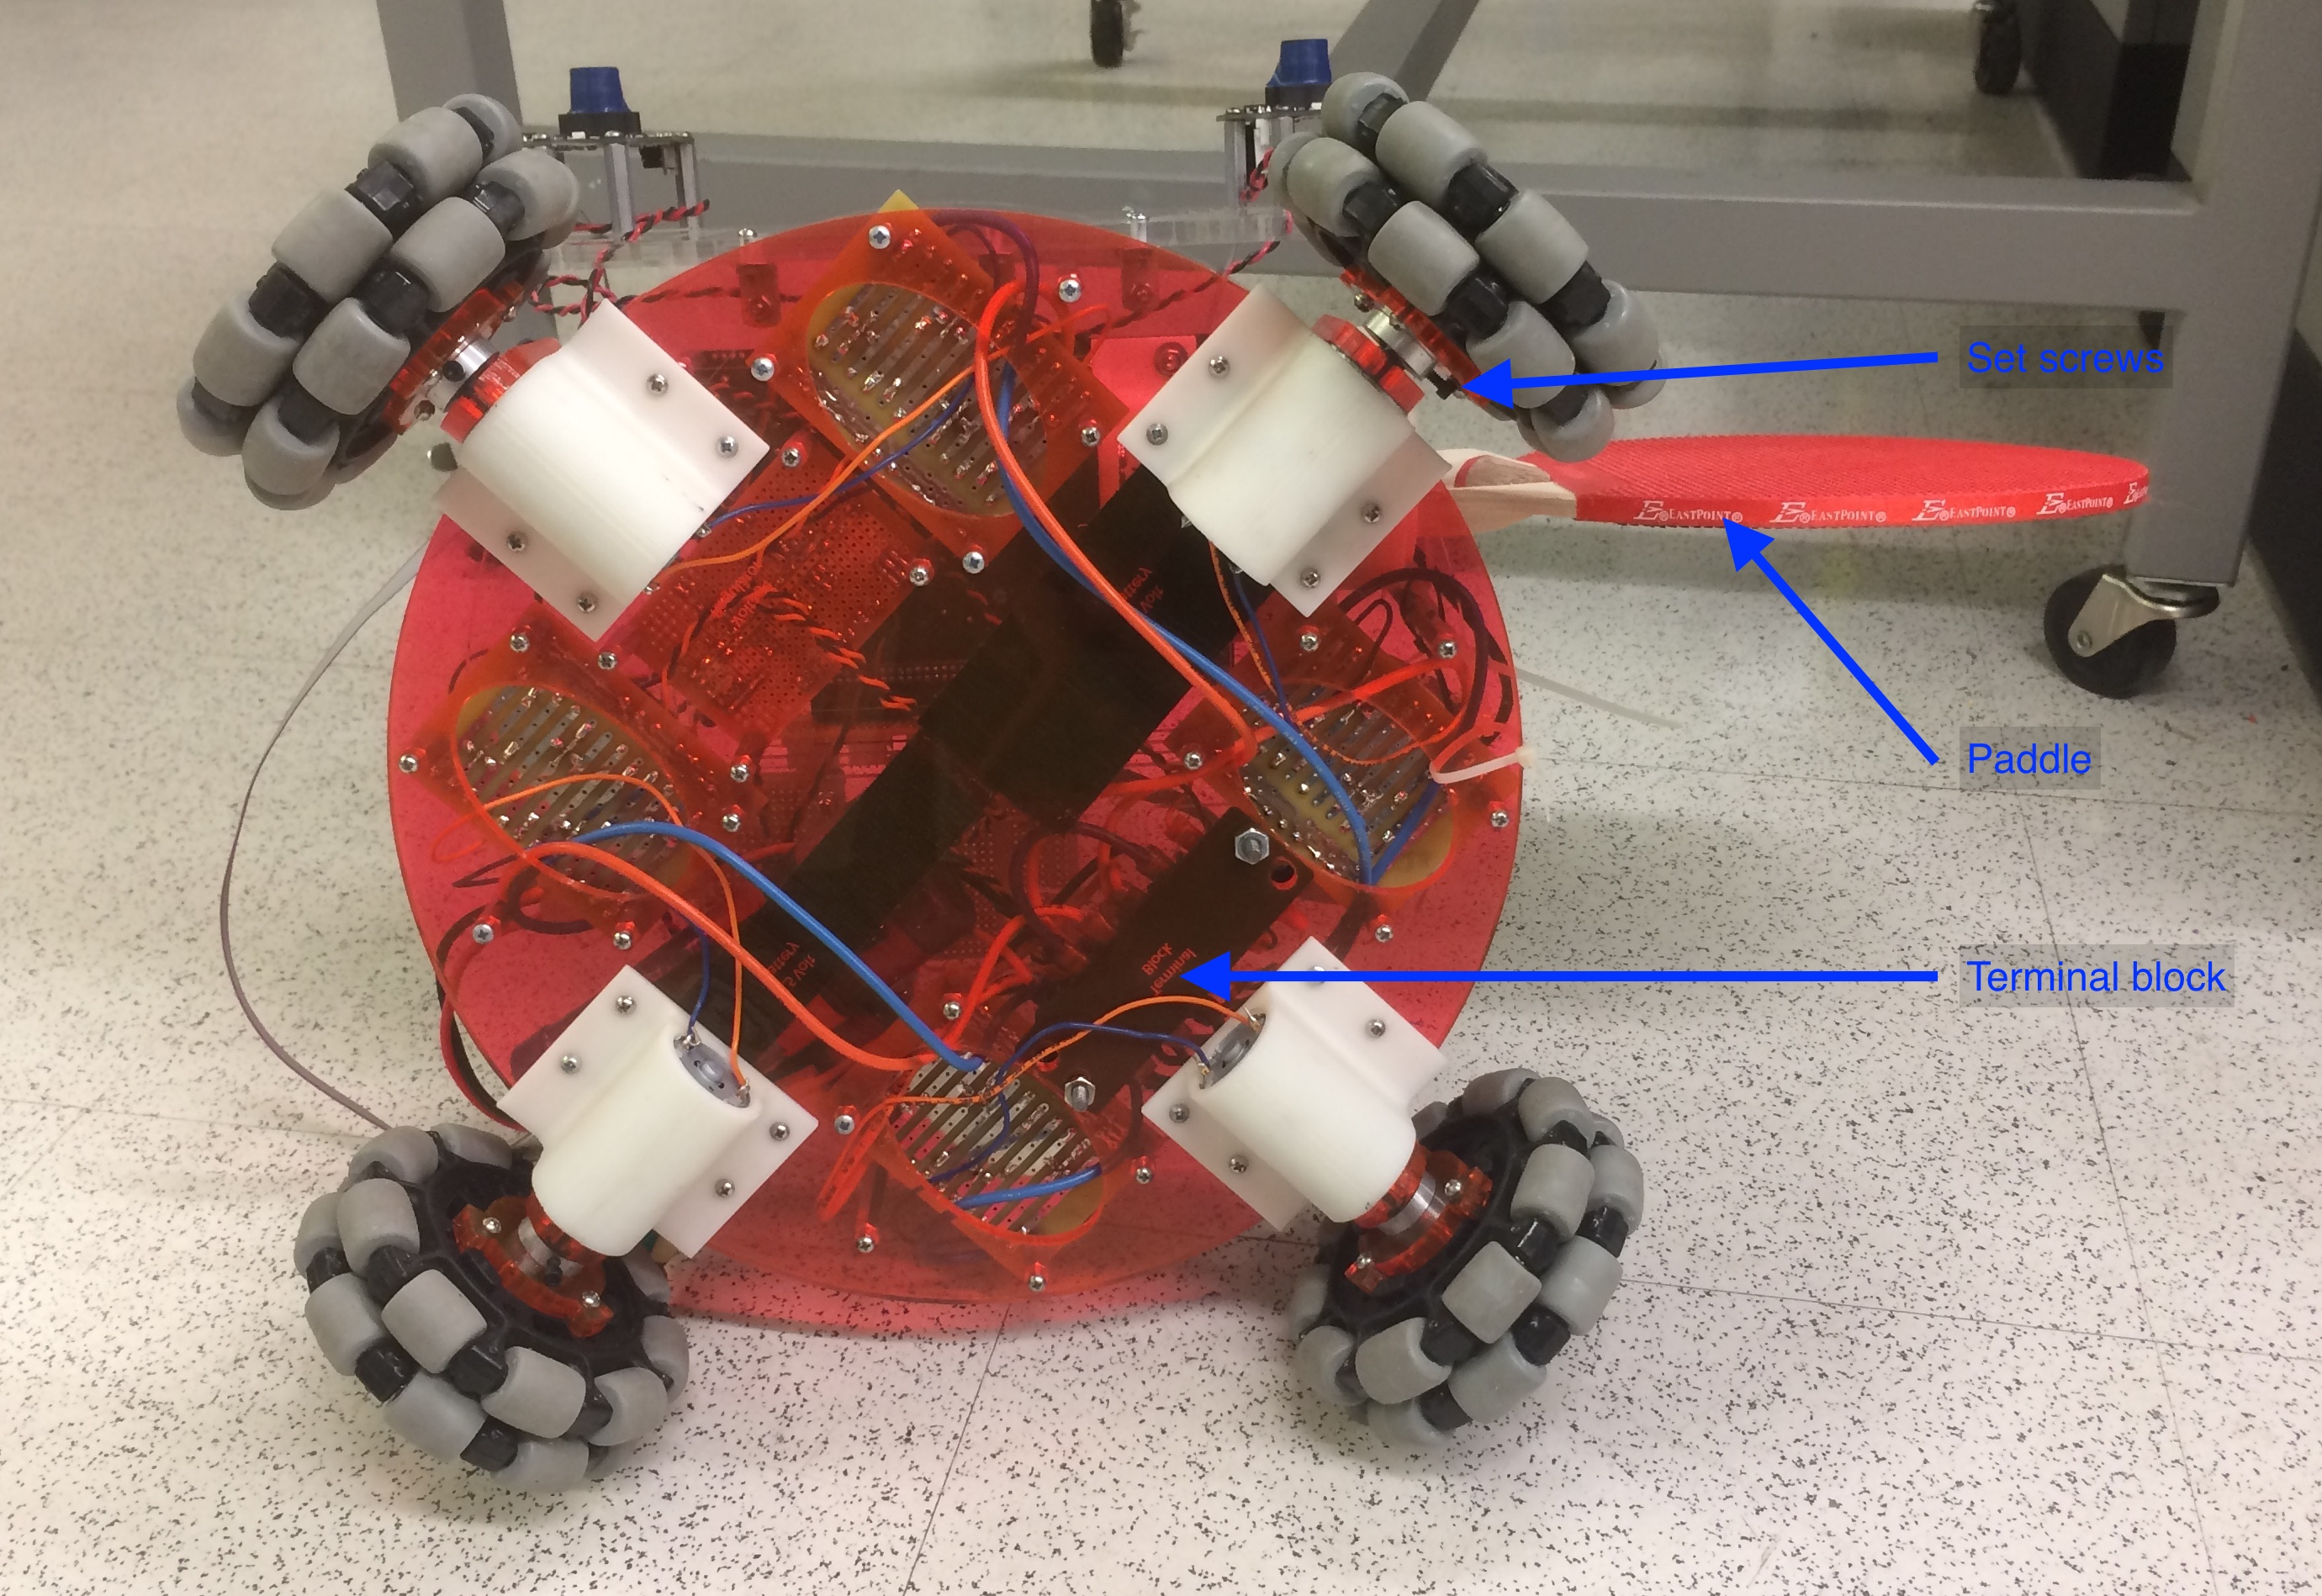
\includegraphics[width=\textwidth]{images/bottom.JPG}
        \caption{Bottom view.}
    \end{subfigure}
\end{figure}

\begin{figure}[H]\ContinuedFloat
    \centering
    \begin{subfigure}[t]{0.8\textwidth}
        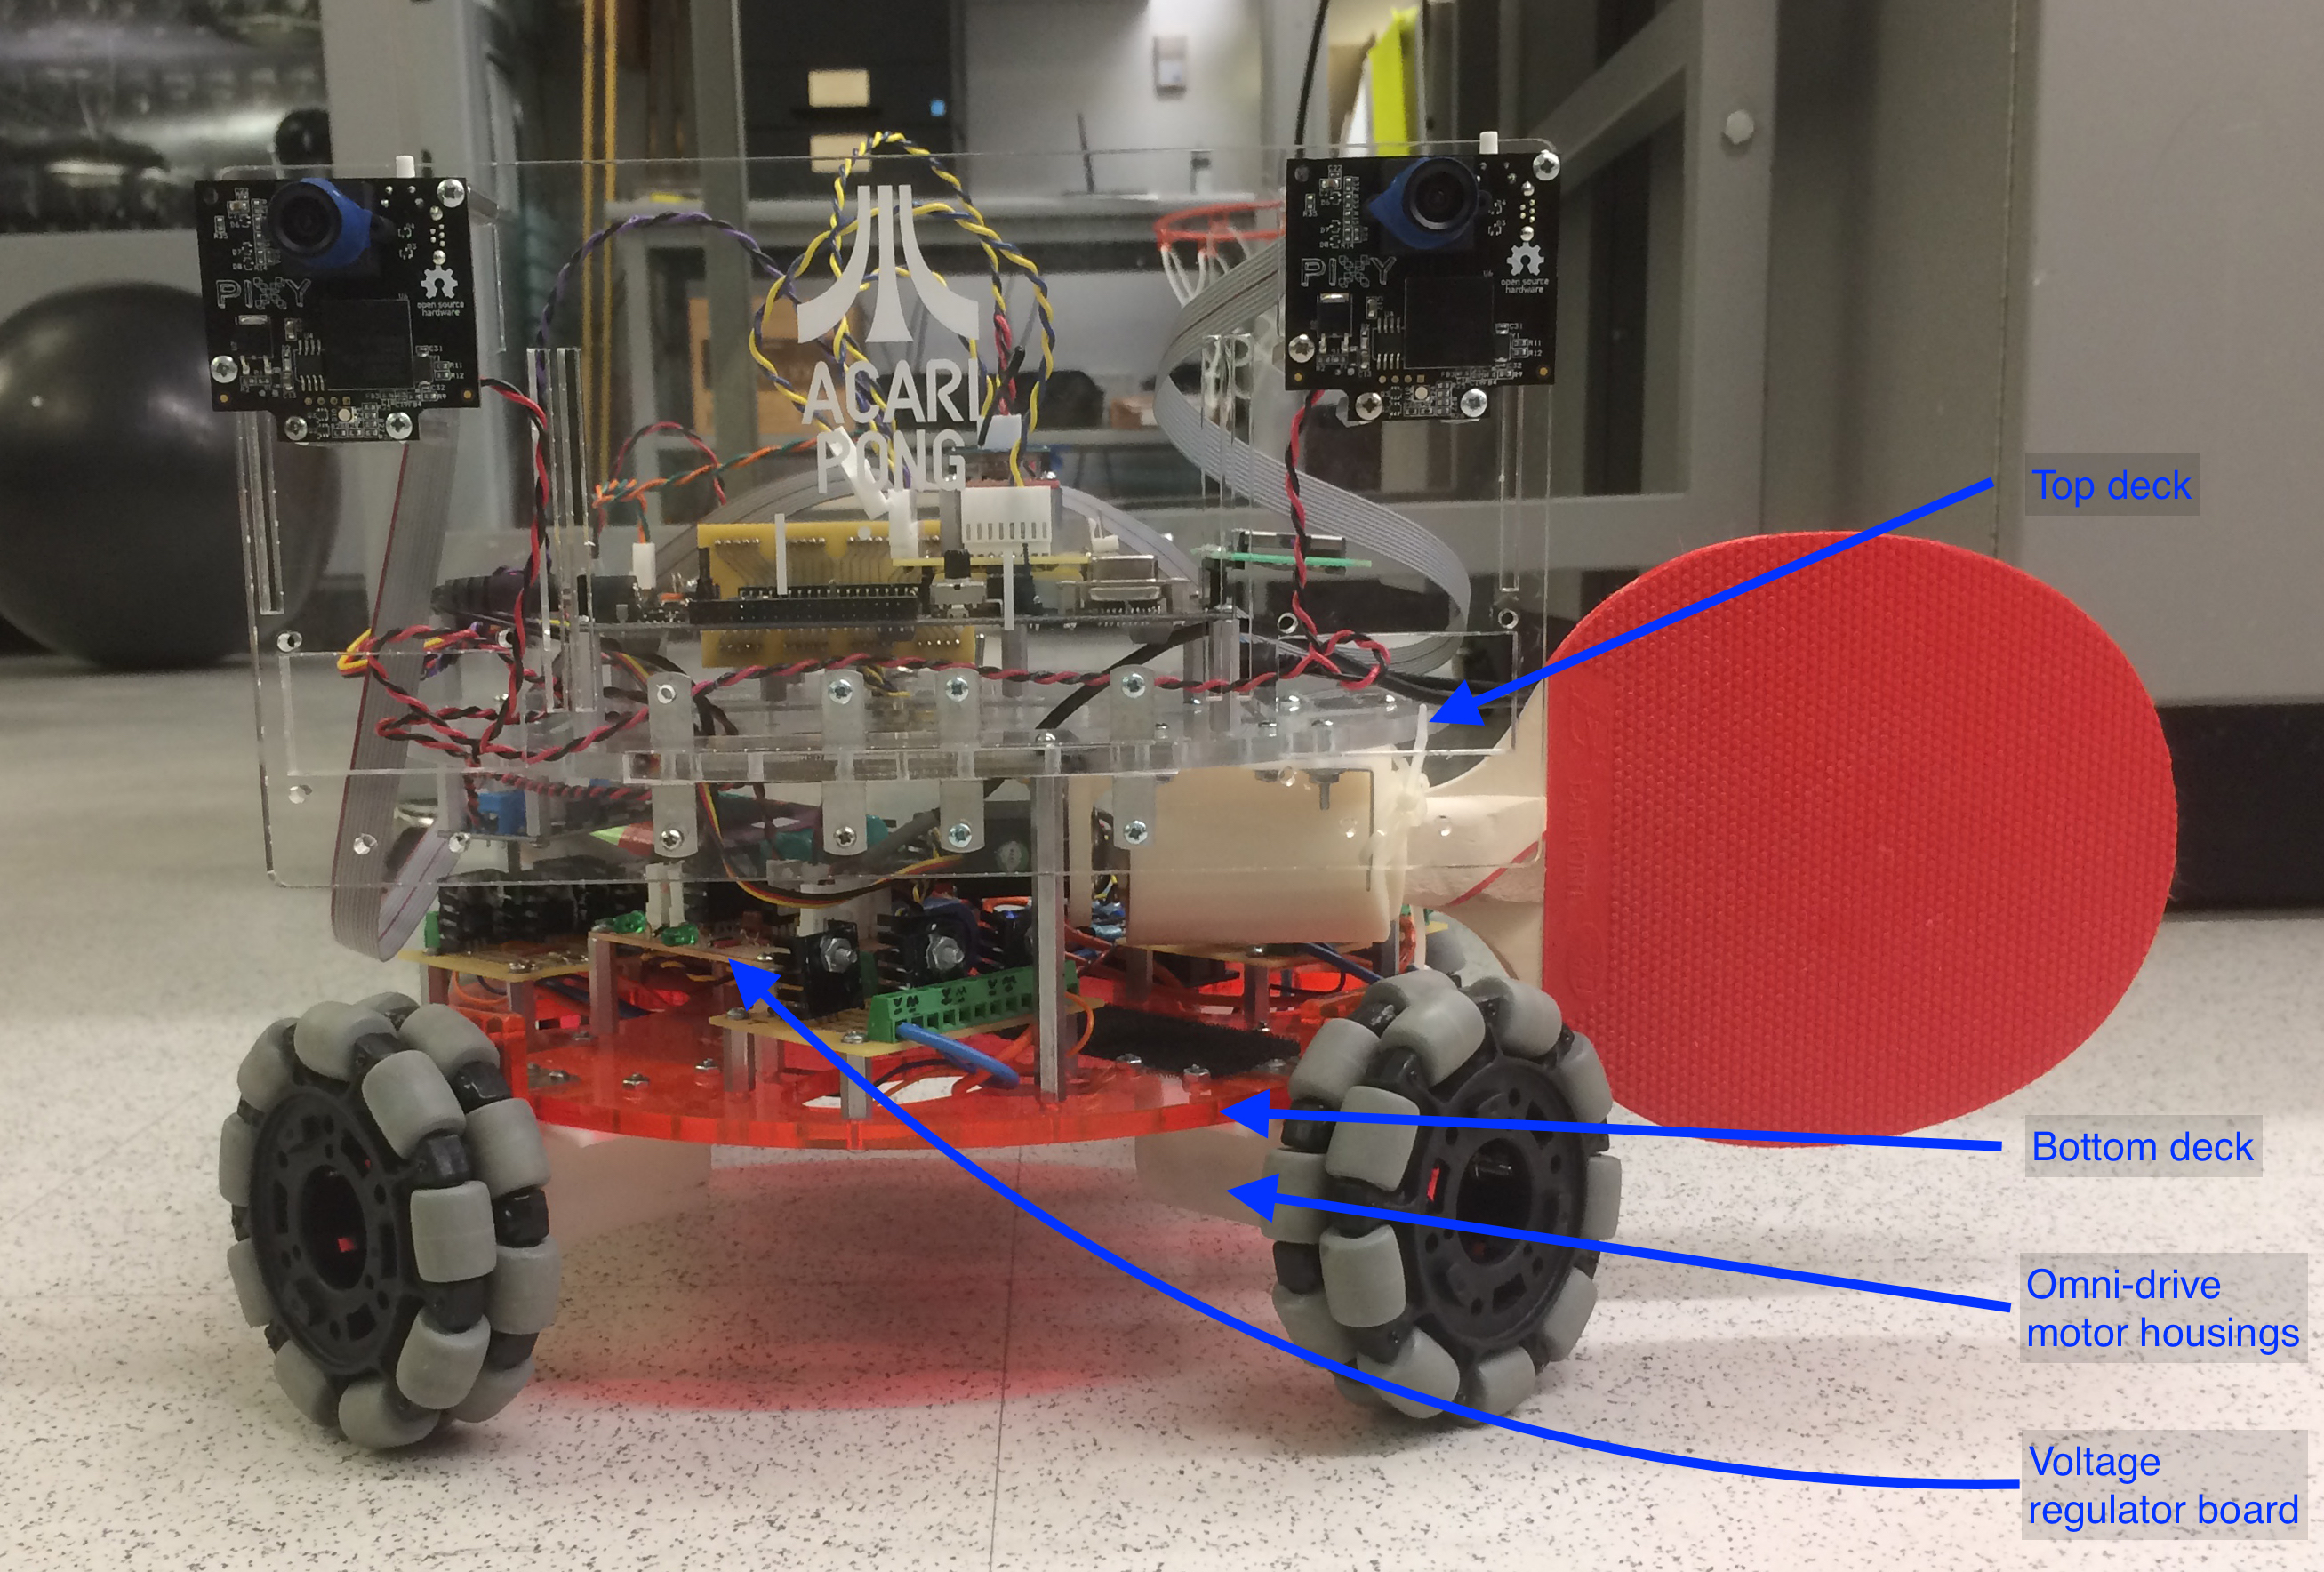
\includegraphics[width=\textwidth]{images/front.JPG}
        \caption{Front view.}
    \end{subfigure}

    \begin{subfigure}[t]{0.8\textwidth}
        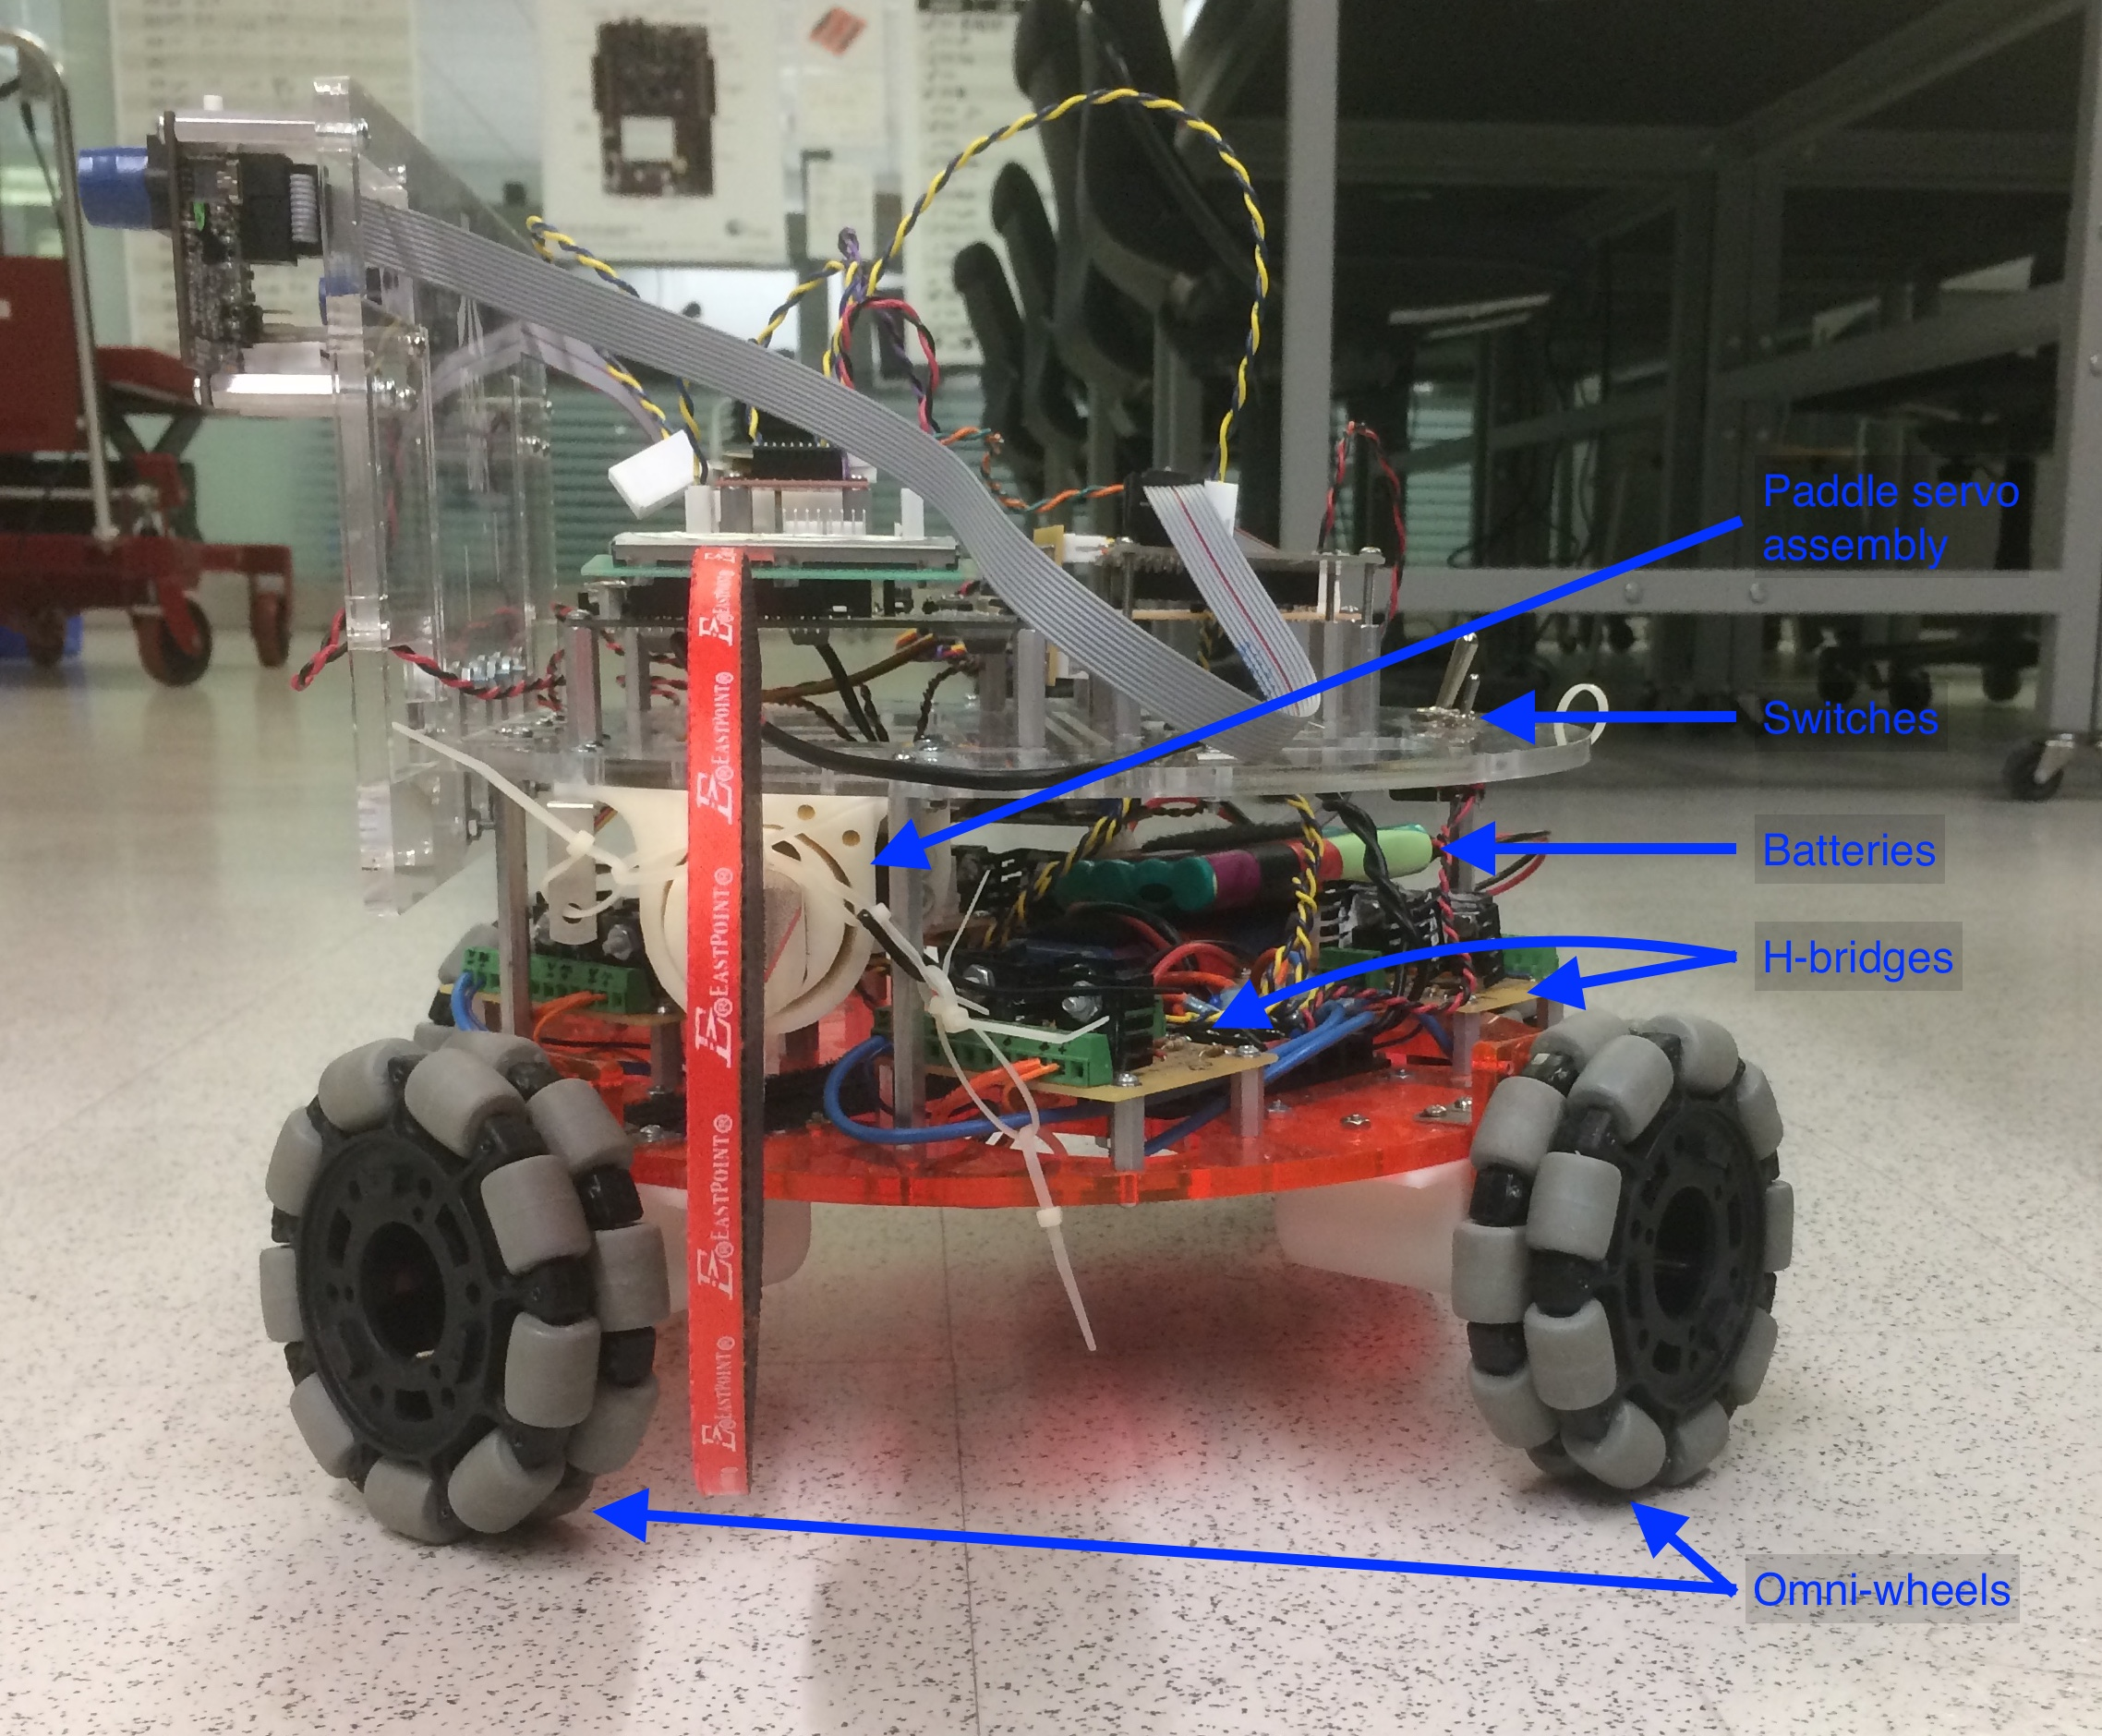
\includegraphics[width=\textwidth]{images/left.JPG}
        \caption{Side view.}
    \end{subfigure}
    \caption{\textbf{Photographs of the final robot.}}
    \label{fig:pics}
\end{figure}
%TODO: BC: block diagram

\figref{fig:blockdiagram} shows a block diagram of the hardware set-up.
\begin{figure}[ht]
    \centering
    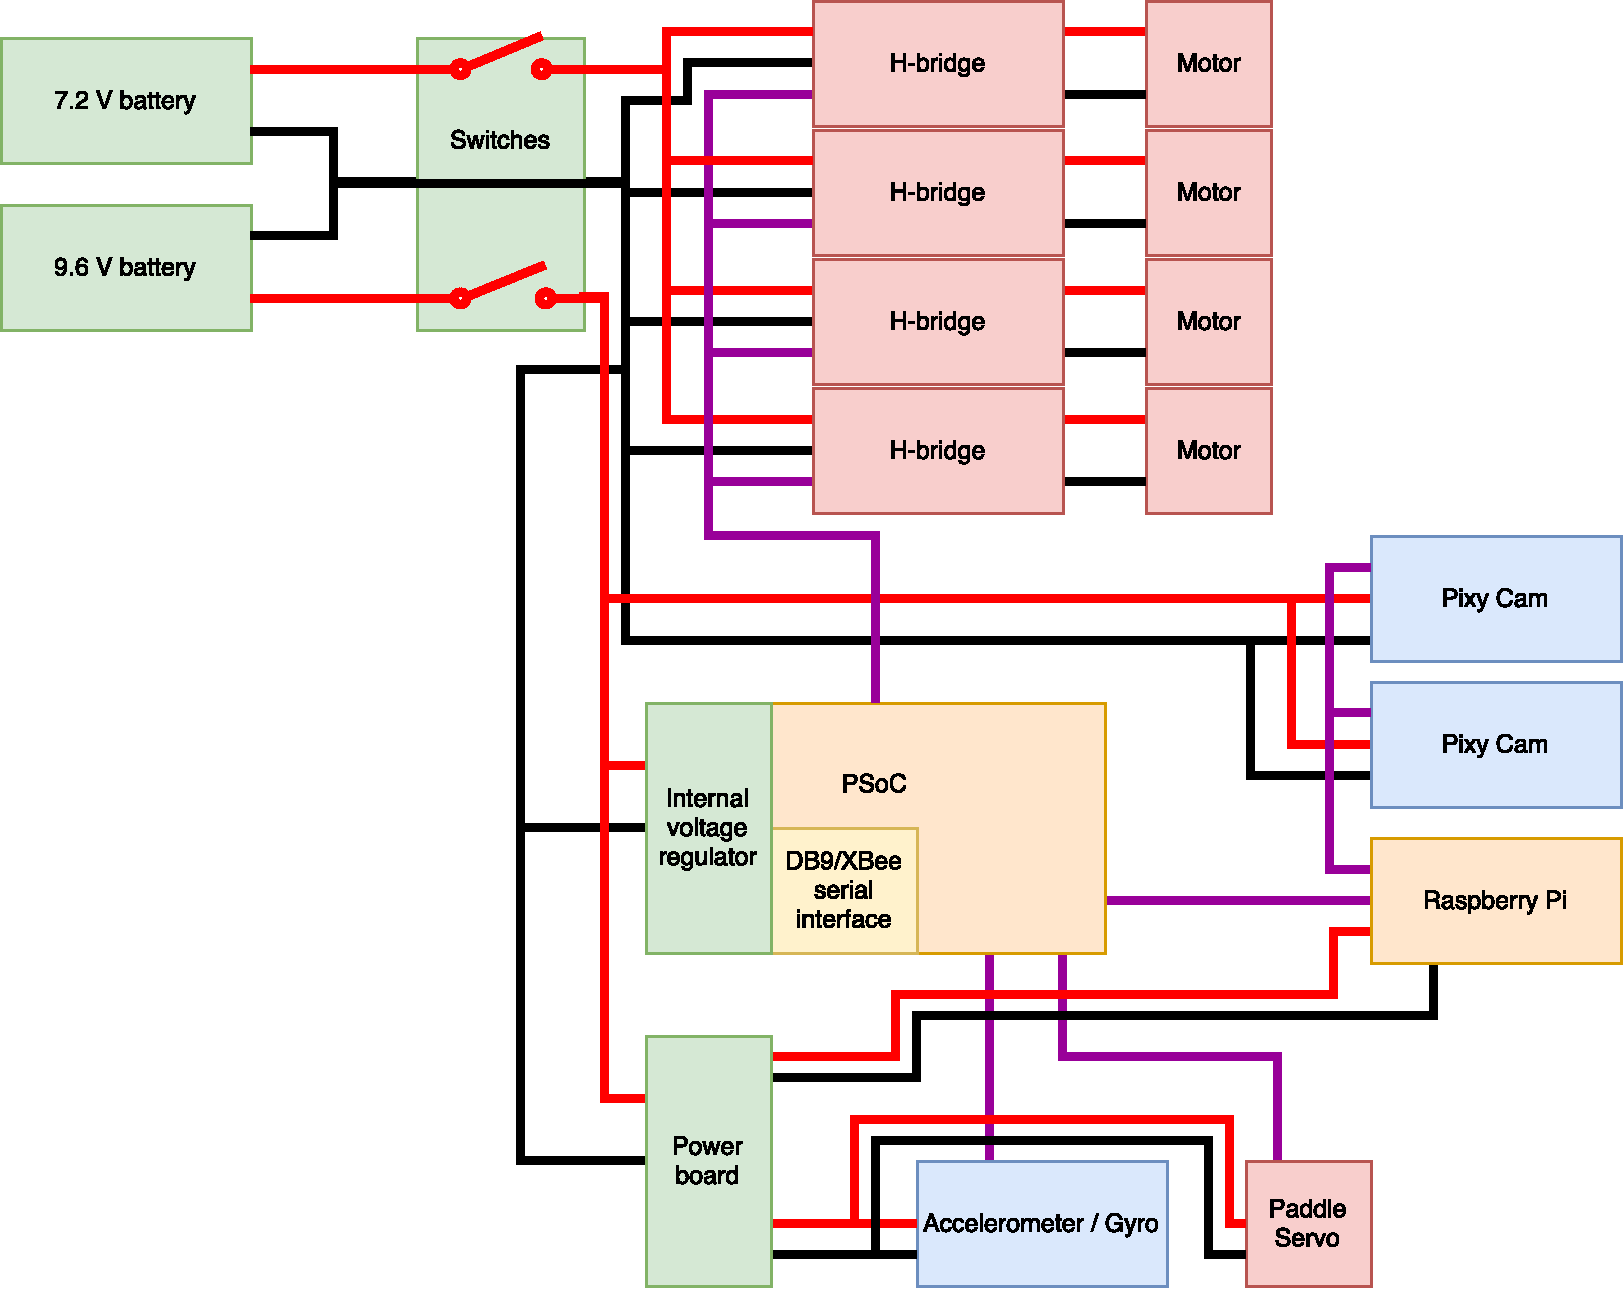
\includegraphics[width=0.85\textwidth]{images/BlockDiagram.pdf}
    \caption{\textbf{Block diagram of the hardware setup for ping pong.} Black connections indicate ground connections; red connections indicate power (both regulated and unregulated); all other connections indicate data connections (e.g. from the PSoC to the H-bridges and servo, various \iic connections). Green components indicate power-related components; red components indicate actuators; blue components indicate sensors.}
    \label{fig:blockdiagram}
\end{figure}

\subsection{Chassis}
%TODO: BC: two decks: lower deck for motors, H bridges, voltage regulator and batteries (we used our own VR because of power requirements); upper deck for RPi, PSoC, accel/gyros
%TODO: BC: figure of laser cut top deck

\subsection{Omni-wheel drive}
%TODO: TJ: what an omni-drive can achieve (i.e. why we needed it), what it requires (independent bidirectional throttled control of four)
\subsubsection{Motors and chassis}
%TODO: TJ: description of motors, chassis (dimensions, components (3D printed components), set screws, etc. - refer to Gordon and Pfleger, 2016), electrical current requirements
\subsubsection{H-bridges and motor control}
%TODO: TJ: description of H-bridges
%TODO: TJ: differences from Gordon and Pfleger (no open-drain comparators)
%TODO: TJ: description of PWM system we used (phase anti-lock? whatever we used)
%TODO: TJ: powered from one 7.2 V NiCd

\subsection{Cameras and mast}
%TODO: BC: camera specifications and details (resoltuion, frame rate, its algorithm and communication protocols)
%TODO: BC: figure of laser cut mast
%TODO: BC: communication protocol

\begin{figure}[ht]
    \centering
    \includegraphics[height=0.3\paperheight,
                     angle=0, origin=c]{images/MastLabeled.jpg}
    \caption{\textbf{Camera mounted on mast.} Labels indicate the mast, the camera and the cable connecting the camera to the camera board.}
    \label{fig:mast}
\end{figure}


\subsection{Paddle mount}
%TODO: TJ: CAD models and servo specifications

\begin{figure}[ht]
    \centering
    \begin{subfigure}[b]{0.45\textwidth}
        \centering
        \includegraphics[height=3in,
                         angle=0, origin=c]{images/CameraBoard.JPG}
        \caption{Photograph}
    \end{subfigure}%
    \begin{subfigure}[b]{0.55\textwidth}
        \centering
        \includegraphics[height=3in,
                         trim=0 0 0 0, clip]{images/CameraBoard.pdf}
        \caption{Schematic}
    \end{subfigure} \\ \vspace{1cm}
    \begin{subfigure}[b]{0.99\textwidth}
        \centering
        \includegraphics[width=\textwidth,
                         trim=0 0 0 0, clip]{images/CameraBoard_circuit.pdf}
        \caption{Circuit diagram}
    \end{subfigure}
    \caption{\textbf{Circuitry of the camera board.}}
    \label{fig:cameraboard}
\end{figure}

\subsection{Power supply}
%TODO: BC: voltage regulators
%TODO: BC: supplying power to the rpi, and difficulties we had

\subsection{Programmable hardware}
%TODO: BC: topdesign
\figref{fig:topdesign} shows the top-design of our programmable hardware in PSoC Creator 2.1.
\begin{figure}[ht]
    \centering
    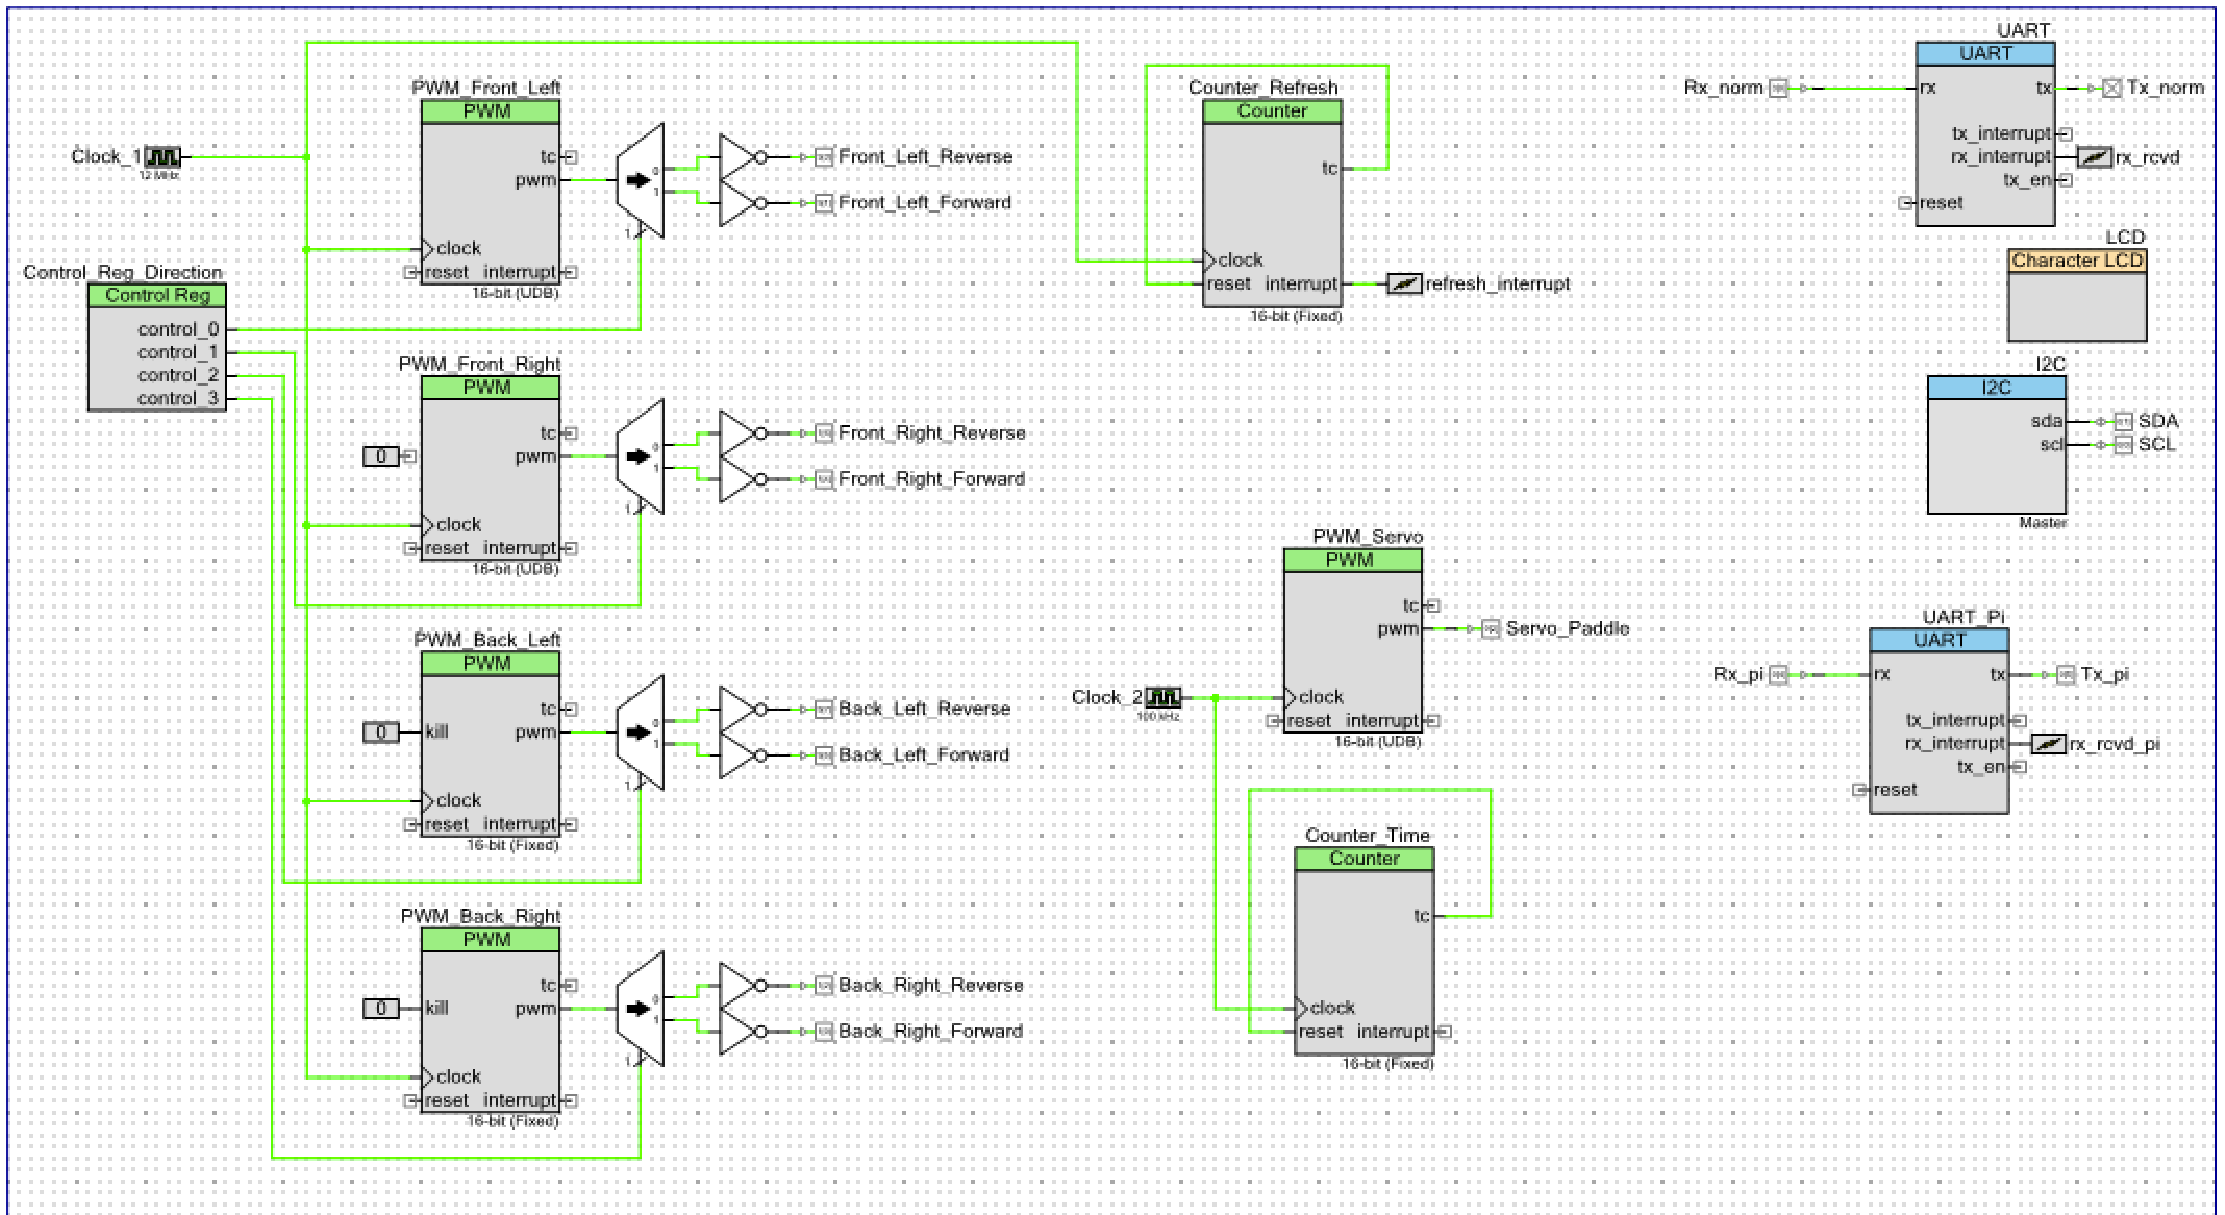
\includegraphics[height=0.99\textwidth,
                     angle=-90, origin=c,
                     trim=1.2in 1in 1.8in 1in, clip]{images/topdesign.pdf}
    \vspace*{-3cm}
    \caption{\textbf{Top-design of the navigation project.}}
    \label{fig:topdesign}
\end{figure}

\subsubsection{Hardware for motor control}
%TODO: TJ

\subsubsection{Hardware for dead reckoning}
%TODO: TJ

\section{Software for PSoC}

\subsection{Omni-drive control}
%TODO: TJ

\subsection{Dead reckoning}
%TODO: TJ

\subsection{Paddle mount servo control}
%TODO: TJ

\section{Software for Raspberry Pi}
\subsection{Pixy camera communication}
%TODO: BC

\subsection{Stereo vision}
%TODO: BC

\subsection{Trajectory estimation}
%TODO: BC

\subsection{Serial communication}
%TODO: update (TJ)
We continued to use serial communication extensively to debug the camera and navigation portions of our program and to adjust our PID variables. We also moved to using the DB9 header only for bench testing and a wireless XBee serial communication chip for track testing. We changed nearly no code or programmable hardware to move to the XBee, since it relied on the same UART communication as the DB9.

We heavily updated our list of serial commands to improve memorability and consistency, and to expand to control camera and navigation parameters. Our updated commands are listed in \tblref{tbl:commands}.
\begin{table}[ht]
    \centering
    \begin{tabular}{@{}ll@{}}
        \toprule
        \textbf{Command} & \textbf{Description} \\ \midrule
        \texttt{CTx} & Change throttle \\
        \texttt{GS} & Get all variables associated with speed control \\
        \texttt{TS} & Toggle speed PID control \\
        \texttt{TDC} & Toggle distance timeout for speed control \\
        \texttt{TDS} & Toggle dynamic speed control \\
        \texttt{CPSx} & Change proportional term for speed control \\
        \texttt{CISx} & Change integral term for speed control \\
        \texttt{CDSx} & Change derivative term for speed control \\
        \texttt{CSSx} & Change steady-state throttle for speed control \\
        \texttt{CTSx} & Change target speed for speed control \\
        \texttt{CTDx} & Change target distance for speed control \\
        \texttt{TVS} & Toggle verbose printout for speed PID control \\ \midrule
        \texttt{GC} & Get all camera variables \\
        \texttt{RC} & Reset camera variables \\
        \texttt{CSx} & Change steering/servo direction \\
        \texttt{CMMx} & Change maximum permitted line misses \\ \midrule
        \texttt{TN} & Toggle navigation PID control \\
        \texttt{CPLx} & Change proportional term for line position error \\
        \texttt{CILx} & Change integral term for line position error \\
        \texttt{CIILx} & Change double integral term for line position error \\
        \texttt{CDLx} & Change derivative term for line position error \\
        \texttt{CPTx} & Change proportional term for angle error \\
        \texttt{CITx} & Change integral term for angle error \\
        \texttt{CDTx} & Change derivative term for angle error \\
        \texttt{CTSNx} & Change nominal target speed for navigation \\
        \texttt{TLE} & Toggle line error tracking \\
        \texttt{TVN} & Toggle verbose printout for navigation PID control \\ \midrule
        \texttt{A} & Abort (kill speed and navigation PID control) \\ \bottomrule
    \end{tabular}
    \caption{\textbf{Table of serial interface commands.}}
    \label{tbl:commands}
\end{table}

\section{Results}
See \tblref{tbl:pid} for the final PID coefficients we used. We updated our coefficients from speed control because we are no longer dynamically updating the target speed to reach the distance in a specific time. We used only the proportional and derivative terms for line position and angle (no integral terms), and unfortunately, despite our efforts to calculate it accurately, the angle contributed very little to our control. Given more time, we may have been able to develop a better system of control to more robustly control steering at higher speeds.
\begin{table}[ht]
    \centering
    \begin{tabular}{@{}rlll@{}}
        \toprule
        & \textbf{P} & \textbf{I} & \textbf{D} \\ \midrule
        Speed control & $80.0$ & $1.0$ & $10.0$ \\
        Line position & $3.0$ & $0.0$ & $2.0$ \\
        Line angle & $0.5$ & $0.0$ & $0.0$ \\ \bottomrule
    \end{tabular}
    \caption{\textbf{Final PID coefficients}}
    \label{tbl:pid}
\end{table}

See \tblref{tbl:times} for our final times for one lap. The highest speed we managed to achieve was with a nominal \SI{6.0}{ft/s}, though by reducing speed while turning corners, our average speed was only about \SI{5.4}{ft/s}. We were unfortunately unable to consistently replicate this speed, and we performed our demo with a nominal target speed of \SI{4.0}{ft/s}.
\begin{table}[ht]
    \centering
    \begin{tabular}{@{}lll@{}}
        \toprule
        \textbf{Nominal target speed} & \textbf{Time for one lap} & \textbf{Average lap speed} \\ \midrule
        \SI{4.0}{ft/s} & \SI{28}{s} & \SI{3.8}{ft/s} \\
        \SI{5.0}{ft/s} & \SI{22}{s} & \SI{4.9}{ft/s} \\
        \SI{6.0}{ft/s} & \SI{19.96}{s} & \SI{5.4}{ft/s} \\ \bottomrule
    \end{tabular}
    \caption{\textbf{Time trial results}}
    \label{tbl:times}
\end{table}

\section{Further work}
%TODO: BC: more robust ball tracking, more robust movement accuracy and location tracking, more robust UART communication, some sort of PID control with global coordinates and camera coordinates so that position could be updated in real time

\clearpage
\section{Appendix: full listings}
\etocsetnexttocdepth{2}
\etocsettocstyle{\subsection*{Contents}}{}
\cftsubsubsecindent 0pt
\localtableofcontents

\subsection{\texttt{main.c}}
% \begin{mdframed}[backgroundcolor=bg]
%     \inputminted[breaklines]{c}{files/main.c}
% \end{mdframed}


\end{document}
